\documentclass[10pt]{amsart}
\usepackage{geometry}                % See geometry.pdf to learn the layout options. There are lots.
\geometry{letterpaper}                   % ... or a4paper or a5paper or ... 
%\geometry{landscape}                % Activate for for rotated page geometry
%\usepackage[parfill]{parskip}    % Activate to begin paragraphs with an empty line rather than an indent
\usepackage{graphicx}
\usepackage{amssymb}
\usepackage{epstopdf}
\DeclareGraphicsRule{.tif}{png}{.png}{`convert #1 `dirname #1`/`basename #1 .tif`.png}

\title{COMP603: Midterm I}
\author{Name: \underline{\hspace{3in}}}
%\date{}                                           % Activate to display a given date or no date

\begin{document}
\maketitle

% Knowledge
% Comprehension
% Application
% Analysis
% Synthesis
% Evaluation

Complete within 120 minutes. Read each question carefully. Write legibly and check your work. No calculators, phones, or laptops are allowed. Good luck!
\section{Short Definitions}
%\subsection{}
Correctly define 8 of the following terms for full credit. Correctly define all for extra credit.\\

\begin{enumerate}
\item String\hfill\underline{}\\\\ %sequence of characters
\item Language\hfill\underline{\hspace{4in}}\\\\ % set of strings
\item Compiler\hfill\underline{\hspace{4in}}\\\\ %translates source language to target language
\item Interpreter\hfill\underline{\hspace{4in}}\\\\
\item Bootstrapping\hfill\underline{\hspace{4in}}\\\\\\\underline{\hspace{5.47in}}\\\\ % writing a compiler in it's own language by first writing a compiler for the language in a different language.
\item Visitor\hfill\underline{\hspace{4in}}\\\\
\item Nondeterminism\hfill\underline{\hspace{4in}}\\\\
\item Ambiguity\hfill\underline{\hspace{4in}}\\\\
\item First set\hfill\underline{\hspace{4in}}\\\\\\\underline{\hspace{5.47in}}\\\\
\item Follow set\hfill\underline{\hspace{4in}}\\\\\\\underline{\hspace{5.47in}}
\end{enumerate}
\section{Lists}
Complete 3 of the following lists for full credit. Complete all for extra credit.\\

\begin{enumerate}
\item Compiler phases, in order. Briefly describe what each phase does.\\\\

\begin{enumerate}
\item \underline{\hspace{5.18in}}\\\\
\item \underline{\hspace{5.18in}}\\\\
\item \underline{\hspace{5.18in}}\\\\
\item \underline{\hspace{5.18in}}\\\\
\item \underline{\hspace{5.18in}}\\
\end{enumerate}

\item Primitive regular expressions. Briefly describe what each regular expression matches.\\\\

\begin{enumerate}
\item \underline{\hspace{5.18in}}\\\\
\item \underline{\hspace{5.18in}}\\\\
\item \underline{\hspace{5.18in}}\\\\
\item \underline{\hspace{5.18in}}\\\\
\item \underline{\hspace{5.18in}}\\\\
\item \underline{\hspace{5.18in}}
\end{enumerate}

\item Finite automaton elements. Describe each. \\\\

\begin{enumerate}
\item \underline{\hspace{5.18in}}\\\\ %set of states
\item \underline{\hspace{5.18in}}\\\\ %start state
\item \underline{\hspace{5.18in}}\\\\ %set of transitions
\item \underline{\hspace{5.18in}}\\\\ % accepting states
\item \underline{\hspace{5.18in}}\\\\ % alphabet
\end{enumerate}

\item For a grammar to be LL(1),\footnote{Left-right, Leftmost derivation, 1 token lookahead} it must be:\\\\

\begin{enumerate}
\item \underline{\hspace{5.18in}}\\\\ % unambiguous
\item \underline{\hspace{5.18in}}\\\\ %free of left recursion
\item \underline{\hspace{5.18in}}\\\\ % free of common prefixes
\item \underline{\hspace{5.18in}} % first (A) disjoint from Follow (A)
\end{enumerate}
\end{enumerate}

\section{Fill in the blank}
Complete the following statements for full credit.\\

\begin{enumerate}
\item A pushdown automaton is a finite automaton with\hfill\underline{\hspace{2.3in}}\\\\
\item A Turing machine is a finite automation with\hfill\underline{\hspace{2.6in}}\\\\
\item It is \underline{\hspace{2in}} possible to define an NFA which cannot be converted into a DFA. 
\end{enumerate}

\section{Regular languages}
Refer to the Figure below. Answer 3 of the following questions. Answer all for extra credit.
\begin{center}
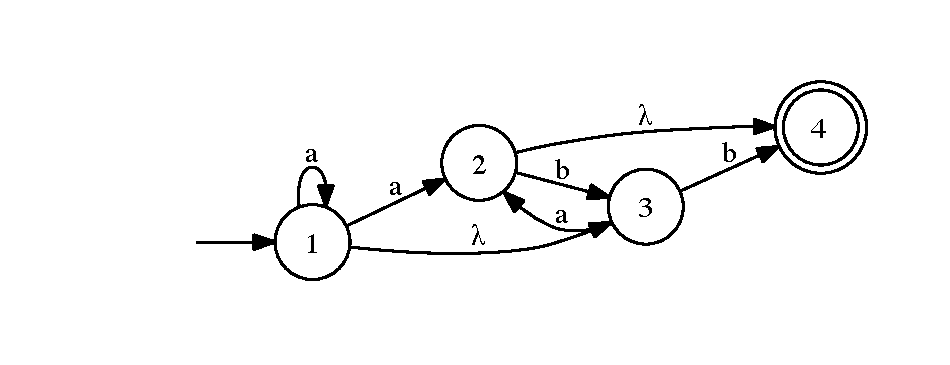
\includegraphics[width=4in]{nfa}
\end{center}
\begin{enumerate}
\item What is the initial state of the DFA using subset construction?\\\\\underline{\hspace{5.18in}}
\item Draw the equivalent DFA using subset construction.\\\\\\\\\\\\\\\\\\\\\\\\\\\\\\\\\\
\item Write the equivalent regular expression.\\\\\\\\\\\\\\
\item IPv4 addresses are written as four integers, separated by dots (e.g., \verb+173.203.204.223+). Each integer ranges from 0 to 255. Write a regular expression to match precisely these addresses.
\end{enumerate}

\section{Context-free languages}
Refer to the context-free grammar below. $S$ is the start symbol. Answer 4 of the following questions. Answer all for extra credit.
\begin{align*}
S &\to T &  T &\to \mathbf{x}\\
S &\to S + T &    T &\to \mathbf{y}\\
S &\to S - T &    T &\to \mathbf{z}\\
S &\to S * T &    T &\to ( S )\\
 S &\to S / T\\
\end{align*}
 \begin{enumerate}
\item Is the grammar above ambiguous? Why or why not?\\\\\\\\\\ % unambiguous
\item Explain why the grammar above is not LL(1).\\\\\\\\\\ % left recursion
\item What is $First(T)$?\\\\\\\\\\ % x, y, z, (
\item What is $Follow(S)$?\\\\\\\\\\ % +, -, *, /, )
\item Perform a leftmost derivation of the following string: $\mathbf{x}*(\mathbf{y}+\mathbf{z})$\\\\\\\\\\\\\\
\end{enumerate}

\section{Extra credit}
Complete any of the following for extra credit.

\begin{enumerate}
\item List all possible $Sentences$ that can be matched by the grammar below.
\begin{align*}
Sentence &\to NounPhrase\ VerbPhrase &     Noun &\to \mathbf{boy}\\
    NounPhrase &\to Article\ Noun    &   Noun &\to \mathbf{ball}\\
    VerbPhrase &\to Verb\ NounPhrase   &  Verb &\to \mathbf{kicked}\\
 Article &\to \mathbf{the}\\ 
\end{align*}
\begin{verbatim}
















\end{verbatim}
\item Rewrite the grammar on the previous page to be LL(1).
\end{enumerate}

\end{document}  